\documentclass[a4paper]{article}
\usepackage{listings}
\usepackage{verbatim}
\usepackage{graphicx}
\usepackage{amsmath}
%% Language and font encodings
\usepackage[english]{babel}
\usepackage[utf8x]{inputenc}
\usepackage[T1]{fontenc}
\usepackage{csvsimple}
%% Sets page size and margins
\usepackage[a4paper,top=3cm,bottom=2cm,left=3cm,right=3cm,marginparwidth=1.75cm]{geometry}

%% Useful packages
\usepackage{amsmath}
\usepackage{graphicx}
\usepackage[colorinlistoftodos]{todonotes}
\usepackage[colorlinks=true, allcolors=blue]{hyperref}

\begin{document}
\begin{titlepage}
	\raggedleft
	\rule{1pt}{\textheight} 
	\hspace{0.05\textwidth} 
	\parbox[b]{0.75\textwidth}{		
		{\LARGE\bfseries EE - 2703 Applied Programming Lab \\[0.5\baselineskip]  ~\huge Assignment -7}\\[2\baselineskip] 
		{\large\textit{The Laplace Transform}}\\[4\baselineskip] 
		{\Large\textbf{Mohammed Khandwawala}}
        \large EE16B117
		\vspace{0.5\textheight}  
	}

\end{titlepage}


\tableofcontents


\section{Introduction}
This assignment is based on analysis Linear-Time invariant systems. Using python signals package of scipy module in python signals impulse response can be analyzed. It is a very powerful package, it allows various operations such as construction transfer function, obtaining its response for any time domain signal and much more.  


\section{Problem -1 : Time Response to spring}
The position of the spring it defined by 
$$ \frac{d^{2}x}{dt^{2}} + 2.25x = f(t) $$
Here f(t) is the forcing function . For this problem f(t) is
$$ f(t) = cos(1.5t)e^{-0.5t}u_{o}(t) $$
Its Laplace transform is given by
$$ F(s) = \frac{s + 0.5}{(s + 0.5)^{2} + 2.25}$$
so from the above equations and the given initial conditions as x(0) = 0 and $\frac{dx}{dt}$ = 0.
X(s) can be written as
$$ X(s) = \frac{s + 0.5}{(s^{2} + s + 2.5)(s^{2} + 2.25)}$$
Inverse Laplace transform of the above expression will time domain position . Using python function impulse from scipy.signal , impulse response of the system can be obtained.  
\begin{lstlisting}[language=Python]
p1 = np.poly1d([1,0.5]) #polynomial s + 1/2
		p2 =: np.poly1d([2,1,2.5]) #polynomial s^2 + s + 5/2
		p3 = np.poly1d([2,0,2.25]) #polynomial s^2 + 2.25
		p2p3 = np.polymul(p2,p3) # multiply p2,p3 (the denominator)
		hs = sp.lti(p1,p2p3)	#numerator divided by denominator (defining transfer funtion)
		t,x = sp.impulse(hs,None,np.linspace(0,50,1000)) #comuting impulse response of the s domain transfer function
		plt.plot(t,x) #plotting time domain signal with x
		plt.xlabel("Time in seconds")
		plt.ylabel("x(t) time domain signal")
		plt.title("solution to d$^{2}$x/dt$^{2}$ + x = cos(1.5t)e$^{-0.5t}u_{o}$(t)")
		plt.show()
\end{lstlisting}
\begin{center}
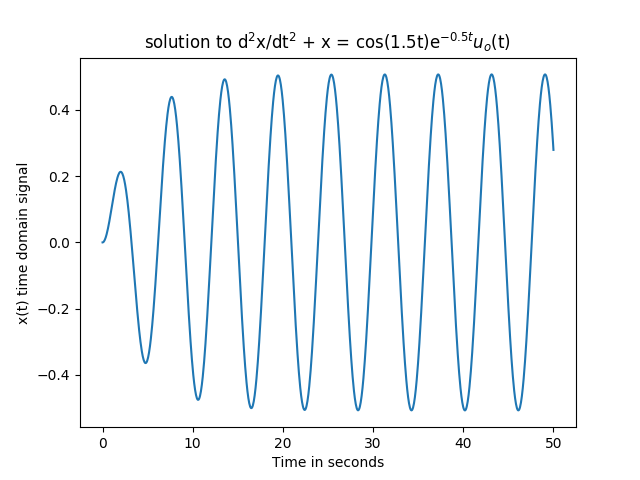
\includegraphics[width=0.8\textwidth]{Figure_1.png}
\end{center}
\subsection{Problem -2 : Response of spring with slower decaying forcing function}
In the second problem which is a subproblem to the first part. The forcing function in this problem is  
$$ f(t) = cos(1.5t)e^{-0.05t}u_{o}(t) $$
In s domain the forcing function is given by
$$ F(s) = \frac{s + 0.05}{(s + 0.05)^{2} + 2.25} $$
This gives X(s) as
$$ X(s) = \frac{s + 0.05}{(s^{2} + 0.1s + 2.2525)(s^{2} + 2.25)}$$
Similarly as in previous problem inverse Laplace transform of the above expression will time domain position . Using python function impulse from scipy.signal , impulse response of the system can be obtained. 
\begin{lstlisting}[language=Python]
p1 = np.poly1d([1,0.05]) #polynomial s + 1/2
		p2 = np.poly1d([2,0.1,2.25+0.0025]) #polynomial s + 1/2
		p3 = np.poly1d([2,0,2.25]) #polynomial s^2 + 1/2
		p2p3 = np.polymul(p2,p3) # multiply p2,p3 (the denominator)
		hs = sp.lti(p1,p2p3) #numerator divided by denominator (defining transfer funtion)
		t,x = sp.impulse(hs,None,np.linspace(0,50,100)) #comuting impulse response of the s domain transfer function
		plt.plot(t,x) #plotting time domain signal with x
		plt.xlabel("Time in seconds")
		plt.ylabel("x(t)")
		plt.title("solution to d$^{2}$x/dt$^{2}$ + x = cos(1.5t)e$^{-0.05t}u_{o}$(t)")
		plt.show()
\end{lstlisting}
\begin{center}
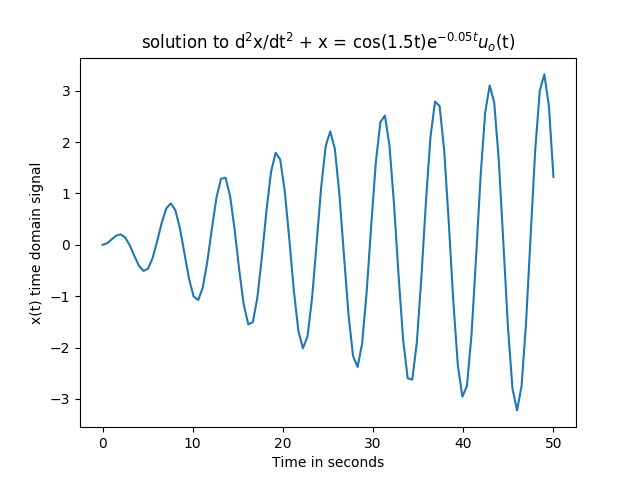
\includegraphics[width=0.8\textwidth]{Figure_2.png}
\end{center}
\subsection{Problem 3: Response of spring to varying frequency of the forcing function}
In this problem the frequency of the forcing function is varied between 1.4 to 1.6  in steps 0.05.
$$ f(t) = cos(\omega*t)e^{-0.05t}u_{o}(t) \hspace{10mm}	1.4 < \omega < 1.6$$
In s domain the forcing function is given by
$$ F(s) = \frac{s + 0.05}{(s + 0.05)^{2} + \omega^{2}}   \hspace{10mm}	1.4 < \omega < 1.6 $$
for this problem scipy.signal's lsim function is used to compute the response from spring system whose transfer function is 
$$ H(s) = \frac{1}{s^{2} + 2.25}$$
lsim takes the transfer function in s domain and input in time domain and returns the time domain output of the system.
\begin{lstlisting}[language=Python]
t = np.linspace(0,50,10000) #calculating for 50 sec
		p1 = np.poly1d([1]) # numerator 1
		p2 = np.poly1d([1,0,2.25])	#denominator polynomial s^2 + 2.25
		H = sp.lti(p1,p2) #numerator by denominator
		for var in np.arange(1.4, 1.6,0.05): #changing frequency of the cosine
			ft = np.cos(var*t)*np.exp(-0.05*t) # input excitation
			t,x,svec = sp.lsim(H,ft,t)  #response of the input excitation
			plt.plot(t,x) #plotting its response
		plt.legend(["1.4","1.45","1.50","1.55","1.6"])	#plot of input response for different frequencies.
		plt.title("Response for different excitaion frequencies.")
		plt.xlabel("Time")
		plt.ylabel("x(t)")	
		plt.show()
\end{lstlisting}
\begin{center}
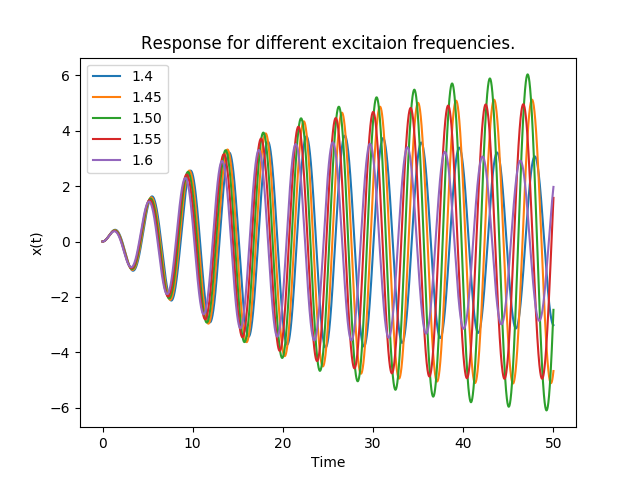
\includegraphics[width=0.8\textwidth]{Figure_3.png}
\end{center}
\begin{center}
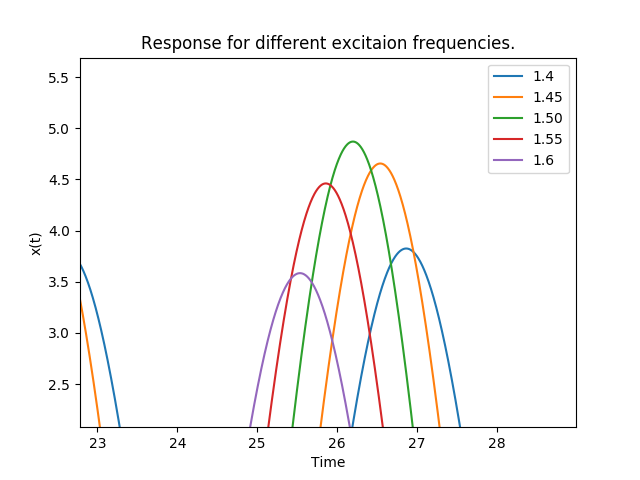
\includegraphics[width=0.8\textwidth]{Figure_3c.png}
\end{center}
Plot of Magnitude and phase response of the spring system which is given by
$$ H(s) = \frac{1}{s^{2} + 2.25}$$.
\begin{lstlisting}[language=Python]
omega,s,phi = H.bode() #plotting phase and magnitude response
		f, axarr = plt.subplots(2,sharex = True)
		axarr[0].set_title("Magnitude Plot")
		axarr.flat[0].set(ylabel = "Magnitude")
		axarr[0].semilogx(omega,s)
		axarr[1].set_title("Phase Plot")
		axarr.flat[1].set(xlabel ="Angular frequency", ylabel = "Phase")
		axarr[1].semilogx(omega,phi)
		plt.show()
\end{lstlisting}

\begin{center}
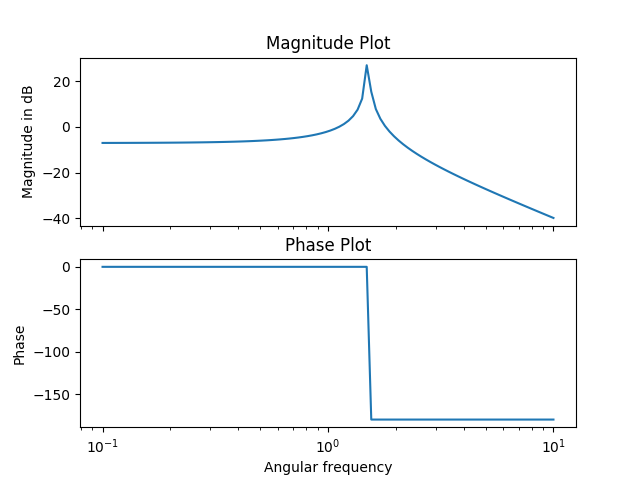
\includegraphics[width=0.8\textwidth]{Figure_3b.png}
\end{center}
From the Magnitude response of the spring mass system the peak occurs at $\omega$ = 1.5. Which matches with observations from the plot of position of the block for different excitation frequencies. Maximum amplitude of oscillation is for $\omega$ = 1.5 which is the natural frequency of the system.
\section{Problem 4 :Coupled Spring Problem}
Positions are described by the given pair of equations
	$$ \frac{d^{2}x}{dt^{2}} + (x - y) = 0$$
	$$ \frac{d^{2}y}{dt^{2}} + 2(y - x) = 0$$
With initial conditions described as $\frac{dx}{dt}_{x=0}$ = 1, $\frac{dy}{dt}_{x=0}$ = 1, x(0) = 0 and y(0) = 0
From the following conditions above X(s) and Y(s) are given by
$$ X(s) = \frac{s^{2} + 2}{s^{3} + 3s}$$
$$ Y(s) = \frac{s^{2}}{s^{3} + 3s}$$
\begin{lstlisting}[language=Python]
#solving coupled equations
		px1 = np.poly1d([1,0,2]) #polynomial s^2 + 2		
		px2 = np.poly1d([1,0,3,0]) #polynomial s^3 + 3s
		X = sp.lti(px1,px2) #transfer function for x
		t1,x = sp.impulse(X,None,np.linspace(0,20,100)) #for 20 sec
		plt.plot(t1,x)
		py1 = np.poly1d([2])	#polynomial 2	
		py2 = np.poly1d([1,0,3,0]) #polynomial s^3 + 3s
		Y = sp.lti(py1,py2)
		t2,y = sp.impulse(Y,None,np.linspace(0,20,100))#for 20 sec
		plt.plot(t2,y)
		plt.xlabel("time")
		plt.legend(["x(t)","y(t)"])
		plt.show()
\end{lstlisting}
\begin{center}
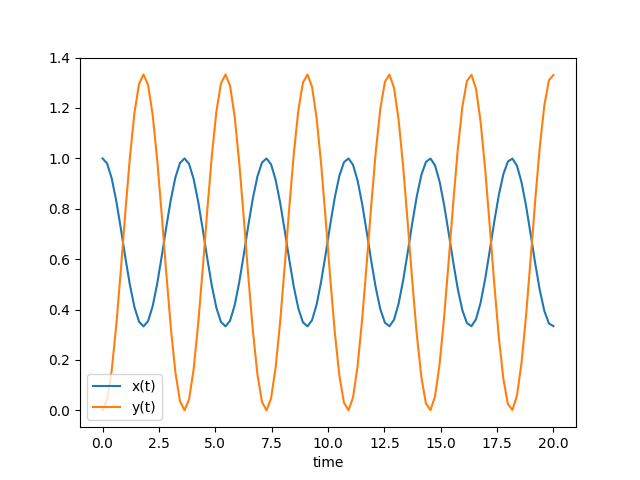
\includegraphics[width=0.8\textwidth]{Figure_4.png}
\end{center}
\section{Problem 5: Magnitude and phase response of RLC circuit }
The transfer function of the RLC network given is given by
$$ H(s)  = \frac{1}{s^{2}10^{-12} + s10^{-4} + 1}$$ 
Using python function Bode to obtain phase and magnitude of any transfer function and plotting it in semi-log scale will give the bode plot of magnitude and phase.
\begin{lstlisting}[language=Python]
px1 = np.poly1d([1]) #numerator 1
		px2 = np.poly1d([1e-12,1e-4,1]) #deominator 10^-12s^2 + 10^-4 +1 
		X = sp.lti(px1,px2) #numerator by denomiantor
		omega,s,phi = X.bode() #plotting frequency and magnitude response
		f, axarr = plt.subplots(2,sharex = True)
		axarr[0].set_title("Magnitude Plot")
		axarr.flat[0].set(ylabel = "Magnitude")
		axarr[0].semilogx(omega,s)
		axarr[1].set_title("Phase Plot")
		axarr.flat[1].set(xlabel ="Angular frequency", ylabel = "Phase")
		axarr[1].semilogx(omega,phi)
		plt.show()
\end{lstlisting}
\begin{center}

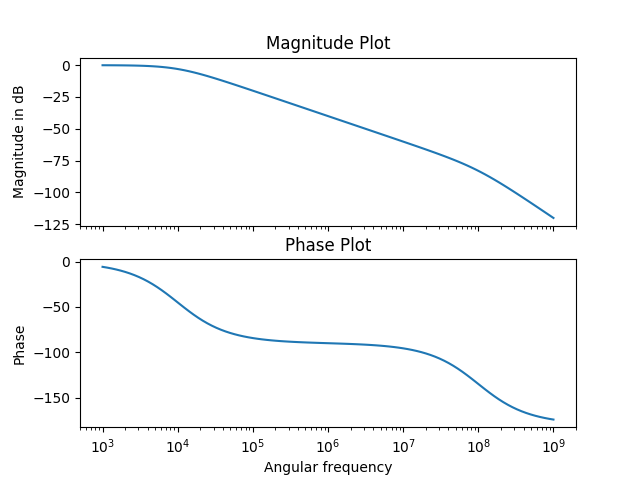
\includegraphics[width=0.8\textwidth]{Figure_5.png}
\end{center}
\subsection{Problem 6: response of RLC network to an input signal }
For a given input voltage signal 
$$ v_{i}(t) = cos(10^{3}t)u(t) - cos(10^{6}t)u(t) $$
The output voltage can be obtained by by scipy.signal's function lsim. It takes transfer function and time domain input and returns output.

\begin{lstlisting}[language=Python]
		#solving for response of rlc network for an input signal cos(10^3t)u(t) - cos(10^6t)u(t)
		px1 = np.poly1d([1])
		px2 = np.poly1d([1e-12,1e-4,1])
		X = sp.lti(px1,px2)
		t1 = np.linspace(0,30e-6,10000) #for time 10ms
		ft = np.cos(1e3*t1)-np.cos(1e6*t1)
		t1,y,svec = sp.lsim(X,ft,t1)
		plt.xlabel("Time")
		plt.ylabel("Output Voltage")
		plt.plot(t1,y)
		plt.show()
\end{lstlisting}
\subsubsection{For simulation up to 10ms}
The given input to RLC network consist of two frequency components , 1K Rad/sec and 1M Rad/sec . Since the RLC network is a low pass filter the out put obtained looks line a sine wave. The Time period obtained from the output is 6.28 ms to which corresponding $\omega$ is 1K Rad/sec . Magnitude Response for this RLC network for $\omega$ = 1K Rad/sec is 0.9090 where as for $\omega$ = 1M Hz it is 0.00980. Hence 1M Hz component of the input is attenuated. The sharp rising is due the transient response and than it becomes close to 1K Rad/sec sine as transient response dies and steady state is reached.
\begin{center}
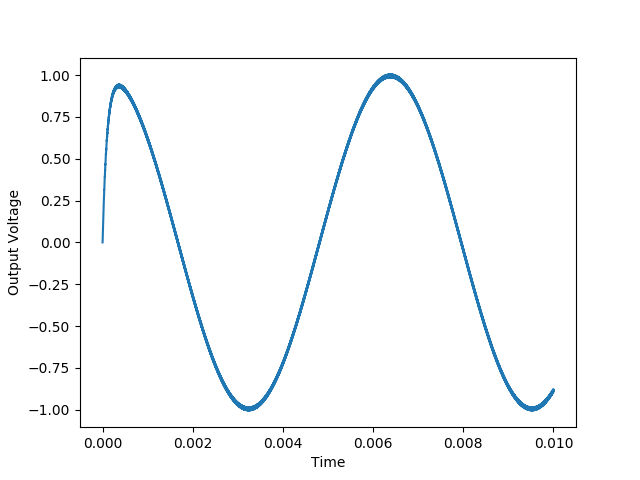
\includegraphics[width=0.8\textwidth]{Figure_6.png}
\end{center}
\subsubsection{For simulation up to 30us}
The simulation from 0 - 30 $\mu$s shows ripples . These ripples are due to the 1M Rad/sec component of the input signal which gets attenuated by the low pass filter. 
\begin{center}
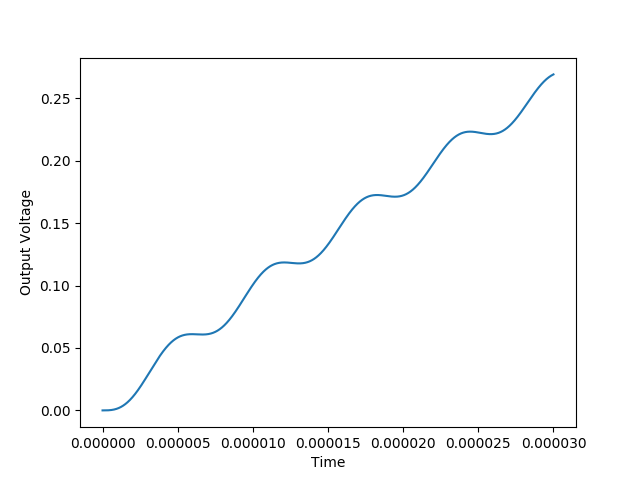
\includegraphics[width=0.8\textwidth]{Figure_6_b.png}
\end{center}
\end{document}

